\documentclass{article}


\usepackage[italian]{babel}
\usepackage[utf8]{inputenc}
\usepackage[T1]{fontenc}
\usepackage{graphicx}
\usepackage{lipsum}
\usepackage{fancyhdr}
\usepackage{titlesec}
\usepackage{tocloft}
\usepackage{titling}
\usepackage{geometry}
\usepackage{float} % Per utilizzare l'opzione H nelle immagini
\usepackage{caption}
\usepackage{multicol} % molteplici colonne


% Formattare codice
\usepackage{listings}
\lstset{language=Python}
\renewcommand{\lstlistingname}{Codice}

% Citazioni 
\usepackage{csquotes}
\usepackage[backend=biber, style=verbose]{biblatex}
\addbibresource{cit.bib}

% Riferimenti
\usepackage[noabbrev]{cleveref}
\crefname{figure}{Figura}{Figure}
\Crefname{figure}{Figura}{Figure}


% Configurazione label immagini
\DeclareCaptionLabelFormat{myformat}{#1~#2}
\captionsetup[figure]{labelformat=myformat}


% Box citazioni
\usepackage{tcolorbox}
\newtcolorbox[auto counter,number within=section]{mybox}[1][]{
    colback=white,
    colframe=black,
    sharp corners, 
    width=0.8\linewidth, 
    center title, 
    title={\textbf{Proprietà (\thetcbcounter)}},
    #1
}


% Margini
\geometry{a4paper, margin=2cm}

% Titolo
\title{Alberi Binari di Ricerca con Chiavi Duplicate}
\author{Niccolò Caselli}
\date{20/01/2024}
\renewcommand{\maketitlehooka}{\centering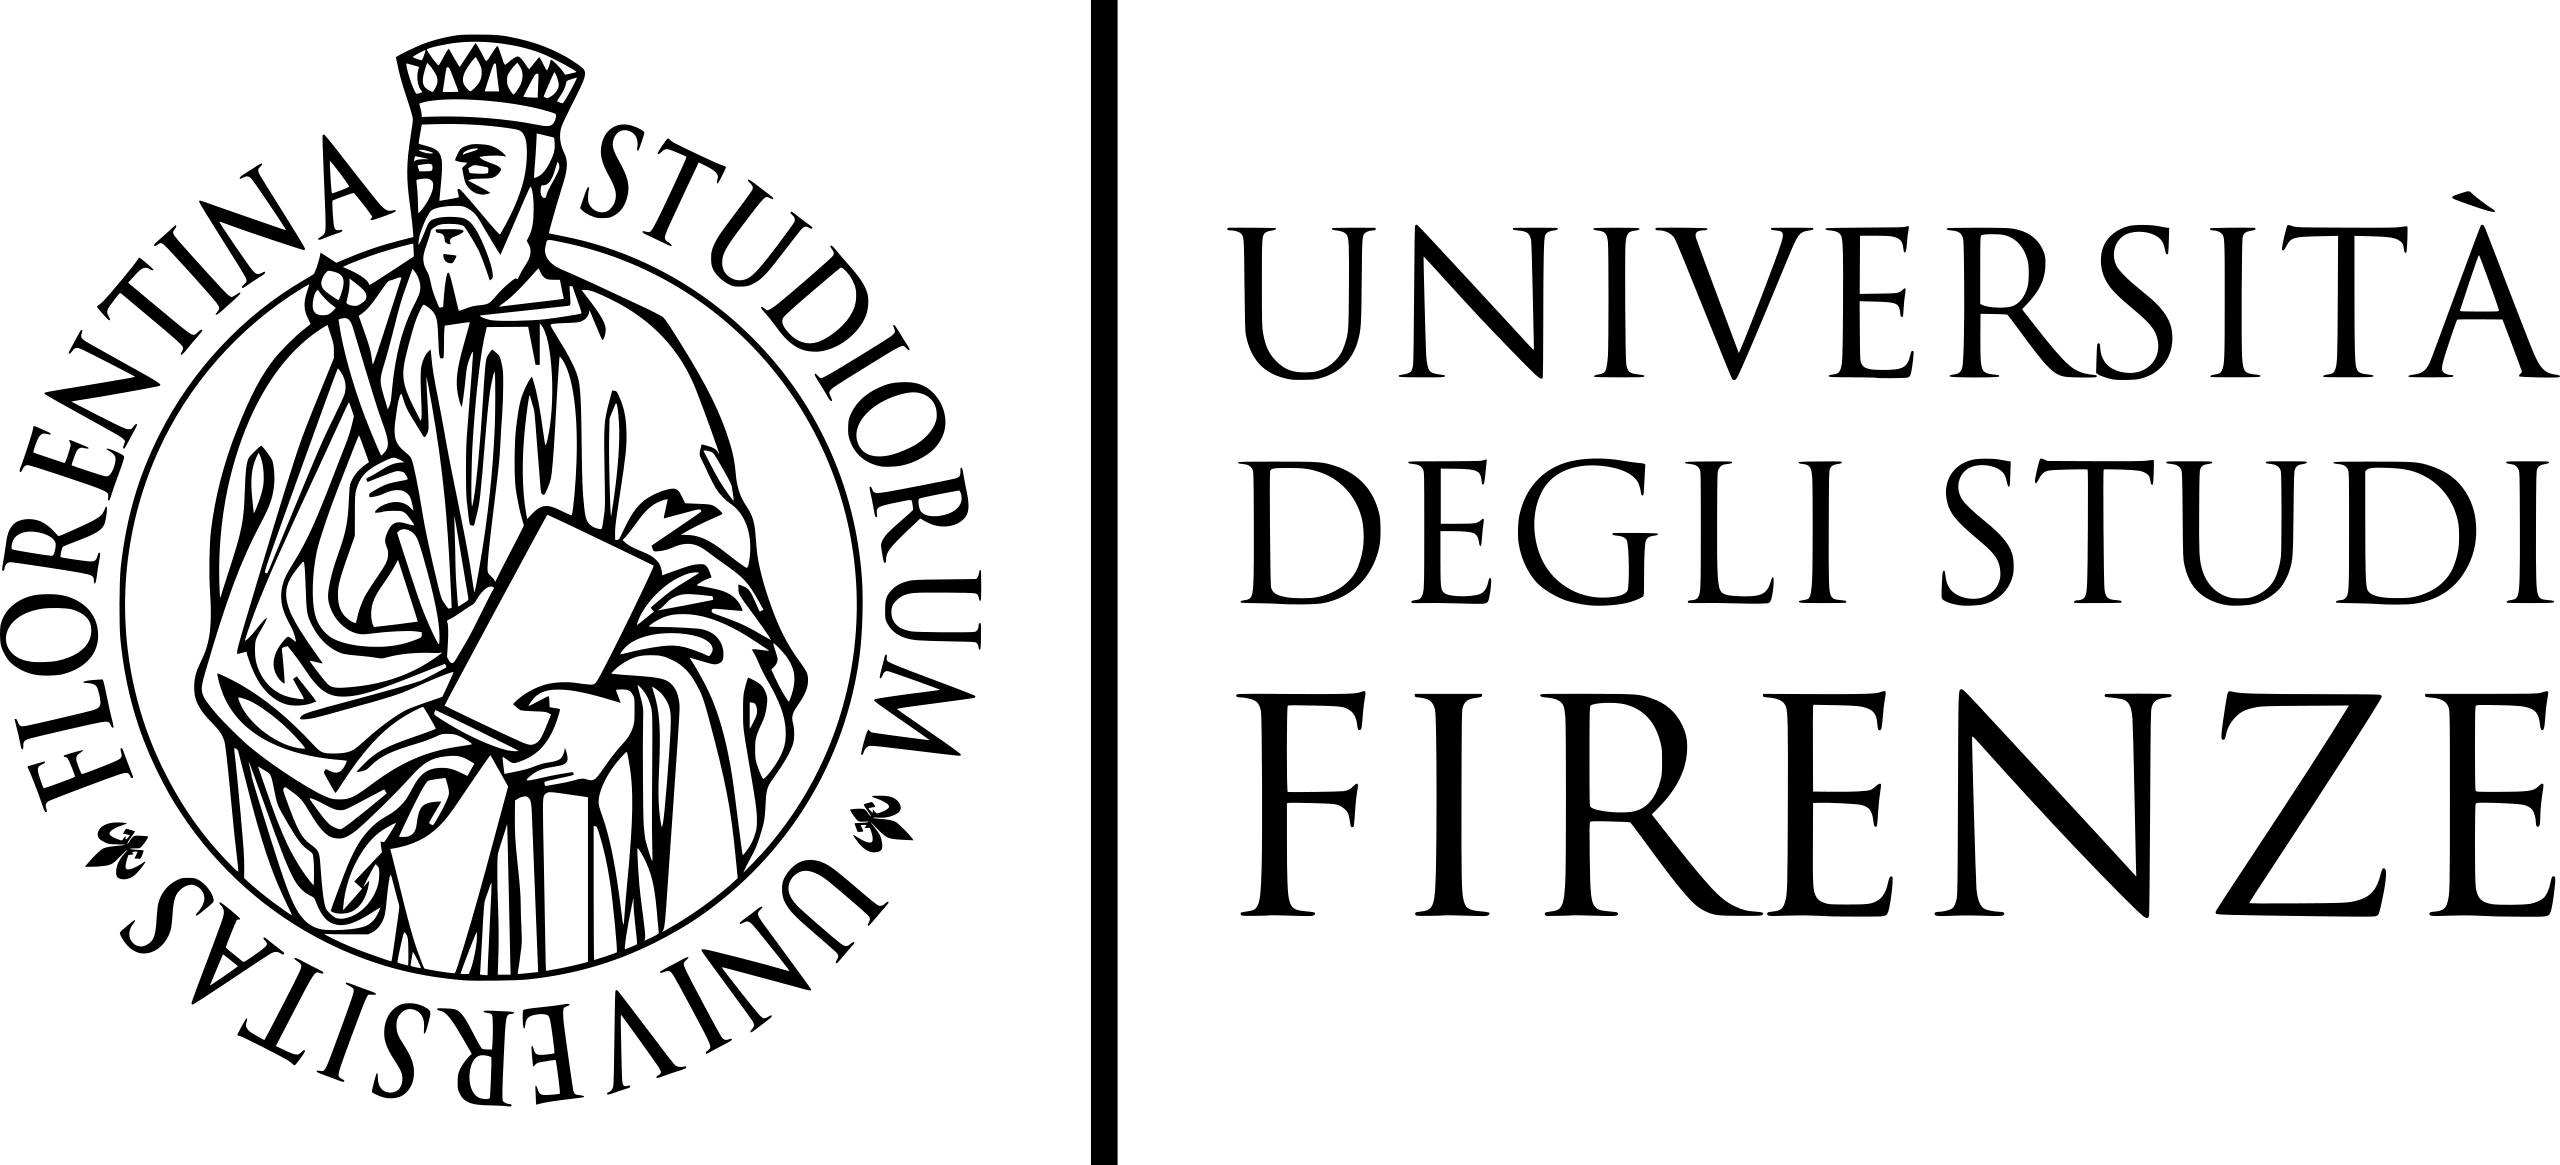
\includegraphics[width=0.5\textwidth]{logo}\vspace{1cm}}
\renewcommand{\maketitlehookb}{\centering\LARGE}
\renewcommand{\maketitlehookc}{\vspace{1cm}\centering\Large}

% Indice
\renewcommand{\cftsecleader}{\cftdotfill{\cftdotsep}}
\setlength{\cftbeforesecskip}{8pt}

% Configurazione degli stili di pagina
\pagestyle{fancy}
\fancyhf{}
\rhead{\thepage}
\lhead{\nouppercase{\leftmark}}
\renewcommand{\headrulewidth}{0.4pt}
\renewcommand{\footrulewidth}{0.4pt}

% Configurazione dei titoli delle sezioni
\titleformat{\section}[block]{\normalfont\Large\bfseries}{\thesection}{1em}{}
\titlespacing*{\section}{0pt}{\baselineskip}{\baselineskip}




\begin{document}

% PAGINA INIZIALE
\begin{titlepage}
  \maketitle
  \vspace*{\fill}
  \begin{center}
    \textbf{Relazione di Laboratorio di Algoritmi e Strutture Dati}
  \end{center}
  \vspace*{\fill}
\end{titlepage}


% INDICE
\renewcommand{\contentsname}{Indice} % Titolo dell'indice
\tableofcontents
\newpage

\section{Introduzione}
\lipsum[1]


\section{Cenni sugli Alberi Binari di Ricerca}

\begin{figure}[H]
  \centering
  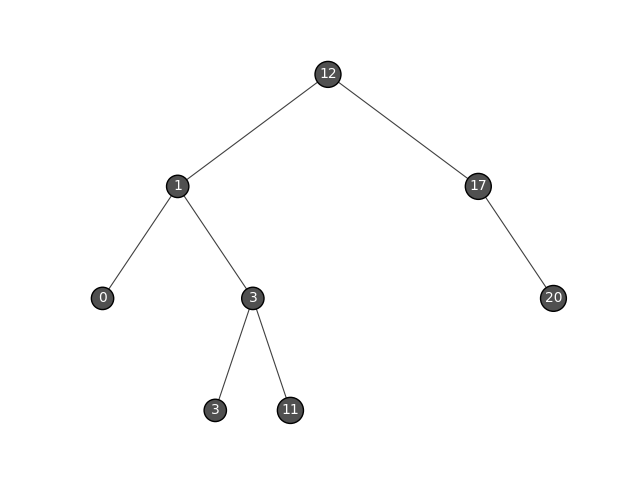
\includegraphics[width=0.7\textwidth]{./images/bst-generic}
  \caption{Esempio di albero binario di ricerca}
  \label{fig:bst-generic}
\end{figure}


\subsection{Cos'è un albero binario di Ricerca?}
\label{subsec:bst-introduction}
Prima di esaminare il problema delle chiavi duplicate cerchiamo di capire cos'è un albero binario di ricerca (abbreviato spesso in B.S.T dall'inglese).
Un BST è un tipo di struttura dati basata su gli alberi, definiti nel libro  \emph{\citefield{cormen2023}{title}} come "grafi non orientati, connessi e aciclici".
Tale struttura ha la caratteristica di permettere le operazioni di base in O(h), con h l'altezza dell'albero, che gli rende efficienti per la realizzazione di dizionari, ricerca di valori, e attraversamenti. \\
Un albero binario di ricerca è costituito da una serie di nodi che nel calcolatore possono essere rappresentati con oggetti con i seguenti attributi:

\begin{itemize}
    \item una chiave (x.key)
    \item un puntatore al figlio sinistro (x.left)
    \item un puntatore al figlio destro (x.right)
    \item un puntatore al padre (x.p)
\end{itemize}

Enunciamo quindi la proprietà fondamentale di un albero binario di ricerca:

\begin{center}
\begin{mybox}
	\begin{itemize}
    \item Se y è nel sottoalbero sinistro di x, allora \(y.key < x.key\) 
     \item Se y è nel sottoalbero destro di x, allora \(y.key > x.key\) 
	\end{itemize}
\end{mybox}
\end{center}
\label{prop:bst-prop} 

Tale caratteristica dei BST è facilmente individuabile nell'albero di esempio di \cref{fig:bst-generic}. 




\subsection{Implementazione in Python}

Come già accennato possiamo rappresentare un albero binario con l'ausilio delle classi. Creiamo quindi una classe per rappresentare l'intero albero e una classe per il singolo nodo dell'albero. Tra queste due classi vi è quindi un relazione 
\textit{one-to-many}.

\vspace{5pt}

\begin{lstlisting}[language=Python, caption={Implementazione di un BST}, label=bst-implementation]


class Node:
    def __init__(self, key):
        self.key = key
        self.left = None
        self.right = None

class BST:
    def __init__(self):
        self.root = None

    # Imposta la radice dell'albero
    def setRoot(self, key):
        self.root = Node(key)

    # Inserisce un nodo nell'albero
    def insert(self, key):
        if (self.root is None):
            self.setRoot(key)
        else:
            self._insertNode(self.root, key)

    # Funzione di supporto per l'inserimento di un nodo
    def _insertNode(self, currentNode, key):
        if (key < currentNode.key):
            if (currentNode.left):
                self._insertNode(currentNode.left, key)
            else:
                currentNode.left = Node(key)
        elif (key > currentNode.key):
            if (currentNode.right):
                self._insertNode(currentNode.right, key)
            else:
                currentNode.right = Node(key)
\end{lstlisting}

\vspace{5pt}

Per ovvi motivi di impaginazione è stato riportato solo parte del codice; il lettore può quindi estenderlo a suo piacere implementando i metodi per gli attraversamenti dell'albero e la ricerca.
Come già sottolineato (Vedi \ref{subsec:bst-introduction}) il vantaggio di questa struttura dati è il costo asintotico delle sue operazioni di base. Più nello specifico, è evidente dalla funzione precedentemente mostrata, l'inserimento in un albero binario è un operazione che richiede $O(h)$ (dal momento che prima di inserire un nuovo nodo bisogna raggiungere una foglia percorrendo al più tutta l'altezza dell'albero - h). Lo stesso discorso si applica per la ricerca e cancellazione (risulta invece diverso il caso degli attraversamenti - in ordine, posticipato e anticipato - che richiedono $\Theta(n)$).
Questo aspetto è fondamentale poiché spiega l'esigenza, su cui torneremo, di avere alberi il più possibili bilanciati. \\
È infine degna di nota la funzione ricorsiva usata nella relazione per la rappresentazione grafica dei BST.

\begin{lstlisting}[language=Python, caption={Rappresentazione Grfaica di un BST}, label=tree-plot]
def plot_tree(tree):
    fig, ax = plt.subplots()
    _plot_tree(ax, tree.root, x=0, y=0, level=1)
    ax.axis('off')
    plt.show()

def _plot_tree(ax, node, x, y, level):
    if node is not None:
        ax.annotate(node.key, (x, y), xytext=(x, y),
                color="white",    
                ha='center',
                va='center', 
                bbox=dict(boxstyle='circle', fc='#505050')
        )

    xfactor = 1/2
    y_new = level * -2

    if node.left is not None:
        x_new = x - xfactor ** level
        ax.plot([x, x_new], [y, y_new], linewidth=.8,color="#404040")
        _plot_tree(ax, node.left, x_new, y_new, level + 1)

    if node.right is not None:
        x_new = x + xfactor ** level
        ax.plot([x, x_new], [y, y_new],  linewidth=.8, color="#404040")
        _plot_tree(ax, node.right, x_new, y_new, level + 1)
\end{lstlisting}


\section{Il Problema delle Chiavi Duplicate}
La definizione data fin'ora di Albero Binario di Ricerca si basa sulla fondamentale supposizione di unicità delle chiavi
(come implicito nella proprietà \ref{prop:bst-prop}).
Sappiamo però che questa ipotesi è difficilmente riscontrabile nelle applicazioni reali:
entriamo, dunque, nel merito del problema delle chiavi duplicate.

Possiamo trovare vari possibili approcci per gestire il problema, in questa relazione ne verranno discussi tre:  



\begin{itemize}
	\item Implementazione \textit{normale} (\ref{subsec:normal-implementation}).
	\item Implementazione con Flag Booleano (\ref{subsec:fag-implementation}).
	\item Implementazione con Lista Concatenata (\ref{subsec:list-implementation}).
\end{itemize}


 
\subsection{Implementazione "normale"}\label{subsec:normal-implementation}
Un primo possibile approccio, e senza dubbi il più immediato, è quello di aggiustare la definizione, volutamente ambigua nel caso di chiavi duplicate, fornita precedentemente (vedi proprietà \ref{prop:bst-prop}).\\
Possiamo quindi riformulare la relazione tra i nodi di un BST affinché supporti l'inserimento quando la chiave da inserire è già presente nell'albero:

\begin{center}
\begin{mybox}
	\begin{itemize}
    \item Se y è nel sottoalbero sinistro di x, allora \(y.key \le x.key\) 
     \item Se y è nel sottoalbero destro di x, allora \(y.key > x.key\) 
	\end{itemize}
\end{mybox}
\end{center}
\label{prop:bst-normal-implementation-prop}

Questa modifica comporta quindi un cambiamento dell'implementazione dell'inserimento nella classe BST: al momento dell'inserimento i nodi con stessa chiave vengono inseriti come figli sinistri del primo nodo con tale chiave (e così via ricorsivamente). Aggiustiamo quindi il codice.

\begin{lstlisting}[language=Python, caption={Funzione ausiliaria di inserimento aggiornata}]
    def _insertNode(self, currentNode, key):
        if (key <= currentNode.key):
            if (currentNode.left):
                self._insertNode(currentNode.left, key)
            else:
                currentNode.left = Node(key)
        elif (key > currentNode.key):
            if (currentNode.right):
                self._insertNode(currentNode.right, key)
            else:
                currentNode.right = Node(key)
\end{lstlisting}

\begin{figure}[htbp]
  \begin{minipage}{0.5\textwidth}
    \centering
    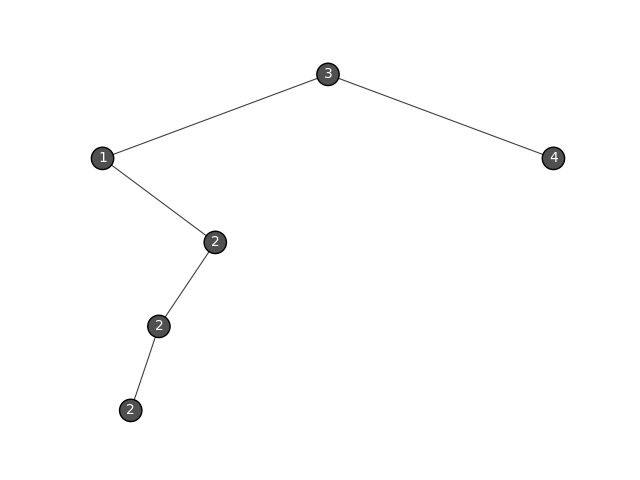
\includegraphics[width=\linewidth]{./images/bst-normal-img1}
    \caption{BST con chiavi duplicate}
    \label{fig:bst-normal-img1}
  \end{minipage}%
  \begin{minipage}{0.5\textwidth}
    \centering
    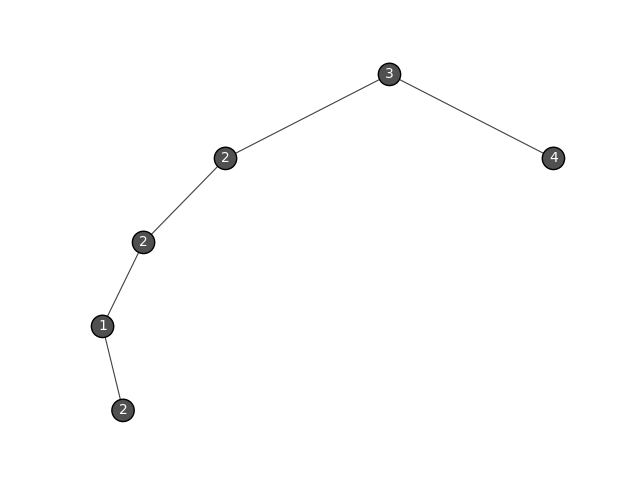
\includegraphics[width=\linewidth]{./images/bst-normal-img2}
    \caption{Altro esempio di BST con chiavi duplicate}
    \label{fig:bst-normal-img2}
  \end{minipage}
\end{figure}



Nella \cref{fig:bst-normal-img1} possiamo vedere l'albero derivante dall'inserimento ordinato dei seguenti elementi \(\mathbf{\{3, 1, 2, 2, 2, 4\}}\). Notiamo quindi che vi sono tre nodi con la stessa chiave 2, ognuno dei quali è nel sotto-albero sinistro del nodo padre più vicino con la medesima chiave.
\\
Non bisogna però cadere nella convinzione che nodi con stessa chiave si trovino sempre tutti adiacenti l'uno con l'altro.
A questo scopo si consideri la \cref{fig:bst-normal-img2}:  cambiando semplicemente l'ordine di inserimento dei valori della figura precedente (ora \(\mathbf{\{3, 2, 2, 1, 2, 4\}}\)) il risultato è molto diverso; tra il penultimo e l'ultimo nodo con chiave 2 vi è in mezzo un nodo con chiave 1!
Questo può portare a complicazioni nella ricerca, che verrà affrontata in seguito. \\

Il principale svantaggio di questa implementazione è che l'inserimento di tante chiavi uguali può tendere a sbilanciare l'albero il quale finisce per degenerare in una semplice lista. Infatti, è evidente che per creare l'albero di N elementi più sbilanciato possibile sia sufficiente inserire N volte la stessa chiave. Come in esempio (\cref{fig:bst-normal-img3}).


\begin{figure}[H]
  \centering
  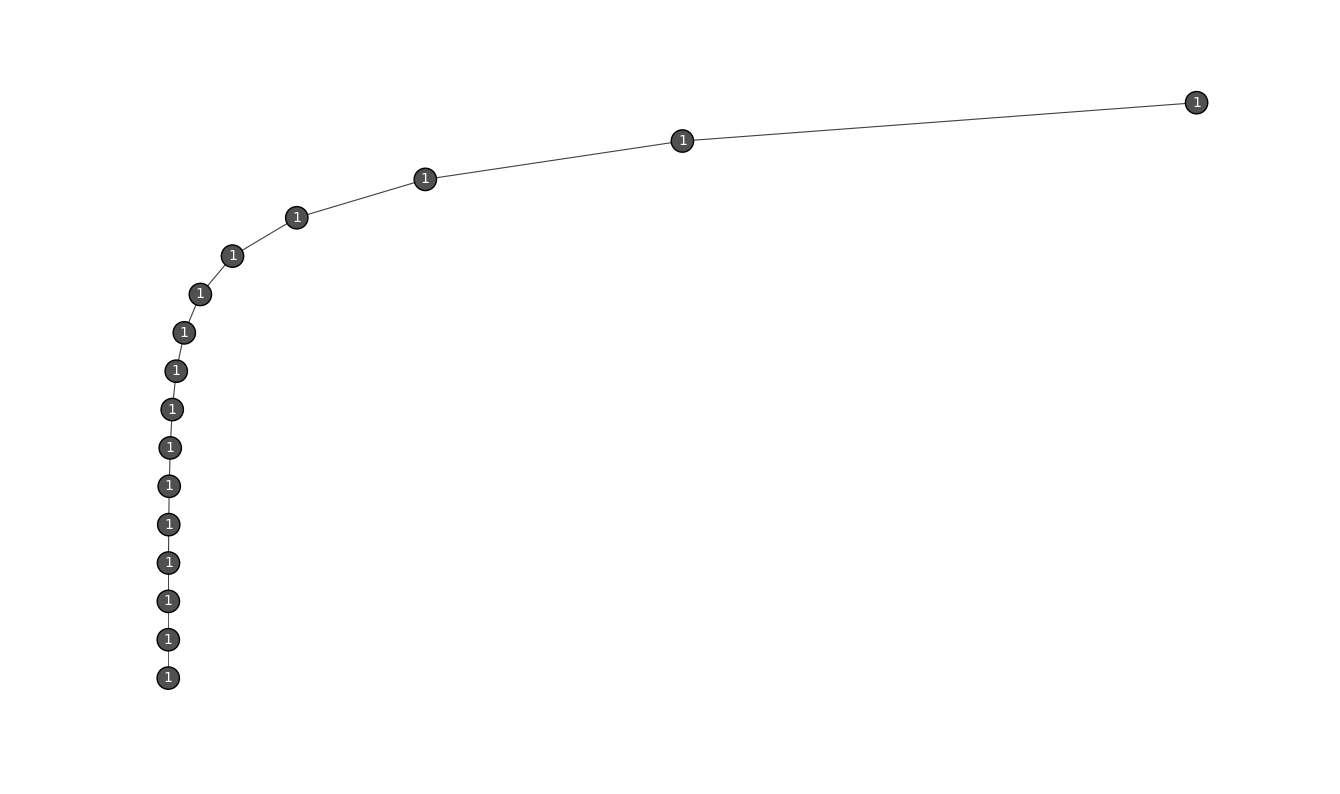
\includegraphics[width=0.7\textwidth]{./images/bst-normal-img3}
  \caption{Esempio di albero binario di ricerca sbilanciato}
  \label{fig:bst-normal-img3}
\end{figure}



\subsection{Metodo del Falg Booleano}
\label{subsec:fag-implementation}

Un altro possibile approccio al caso delle chiavi duplicate è, invece di inserire sempre i nodi con chiave duplicate a sinistra del nodo padre, inserire i nodi con chiave duplicate a sinistra o destra del padre a seconda di un flag booleano. Più nello specifico: estendiamo la struttura dati di ogni nodo dell'albero così che il generico nodo x abbia un nuovo attributo \textit{x.flag} e quindi, durante l'inserimento, porre x a \textit{x.left} o \textit{x.right} a seconda del valore del flag, il quale viene alternato a ogni visita di x con chiave uguale. 

Il punto di forza di questa implementazione è il fatto che tende a preservare il bilanciamento dell'albero anche in presenza di molte chiavi duplicate, a differenza del primo approccio (Vedi \ref{subsec:normal-implementation}). Ciò risulta evidente se si prova a disegnare l'albero risultante dall'inserimento di N chiavi uguali (Vedi \cref{fig:bst-flag}).



\begin{figure}[H]
  \centering
  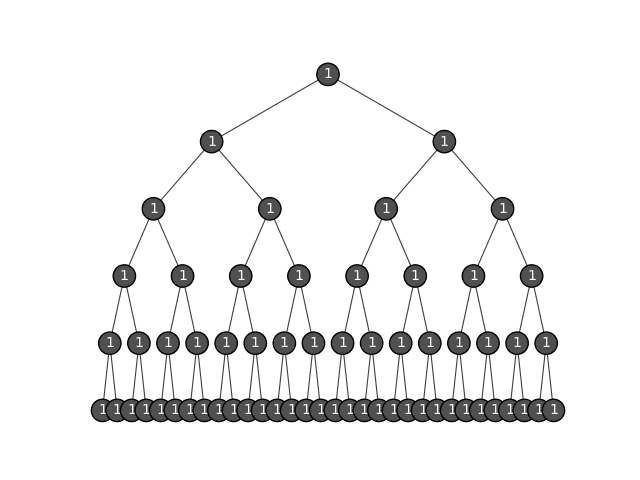
\includegraphics[width=0.7\textwidth]{./images/bst-flag}
  \caption{BST con Flag Booleano di 64 chiavi uguali}
  \label{fig:bst-flag}
\end{figure}



Per quanto riguarda il codice, le modifiche da apportare sono minime.
Aggiungiamo il nuovo attributo nella classe Nodo:

\begin{lstlisting}[language=Python]
class Node:
    def __init__(self, key):
        self.key = key
        self.left = None
        self.right = None
        self.flag = False # <---
\end{lstlisting}

E aggiorniamo la funzione di supporto per l'inserimento:

\begin{lstlisting}[language=Python]
    def _insertNode(self, currentNode, key):        
        if(currentNode.key == key):
            if(currentNode.flag): self._insert_right(currentNode, key)
            else: self._insert_left(currentNode, key)
            currentNode.flag = not currentNode.flag # Alterna il flag
    
        if (key < currentNode.key): self._insert_left (currentNode, key)
        elif (key > currentNode.key): self._insert_right(currentNode, key)

    # Funzione di supporto per l'inserimento di un nodo a sinistra
    def _insert_left(self, currentNode, key):
        if (currentNode.left): self._insertNode(currentNode.left, key)
        else: currentNode.left = Node(key)

    # Funzione di supporto per l'inserimento di un nodo a destra
    def _insert_right(self, currentNode, key):
        if (currentNode.right): self._insertNode(currentNode.right, key)
        else: currentNode.right = Node(key)
\end{lstlisting}











\subsection{Metodo della Lista Concatenata}
\label{subsec:list-implementation}




\section{Test delle prestazioni}
\subsection{Analisi Teorica}
\subsection{Risultati Sperimentali}
\newpage

% PC 
\section*{Nota sui test}
\addcontentsline{toc}{section}{Nota sulle Caratteristiche del Computer}


Si tenga presente svolgere i test discussi è necessario alzare il limite massimo di ricorsione di default di Python. Questo è necessario per prevenire che l'interprete blocchi l'esecuzione di un elevato numero di chiamate ricorsive, però necessarie in questa tipologia di test.
Per fare ciò basta impostare un nuovo limite nel seguente modo:
\begin{lstlisting}[language=Python]
sys.setrecursionlimit(500000000)
\end{lstlisting}


\vspace{20pt}


Si tenga inoltre presente che tutti i test presenti in tale relazione sono stati eseguiti su un calcolatore con le seguenti specifiche:

\begin{multicols}{2}
    \textbf{Hardware:}
    \begin{itemize}
        \item \textbf{Modello:} MacBook Pro 2022
        \item \textbf{CPU:} Apple Silicon M2 (8 core)
        \item \textbf{RAM:} 8 GB LPDDR5 (Micron)
    \end{itemize}
    
    \columnbreak
    
    \textbf{Software:}
    \begin{itemize}
        \item \textbf{Versione macOS:} 14.0
        \item \textbf{Versione Python:} 3.11.4
        \item \textbf{Versione Pip3:} 23.3.2
    \end{itemize}
\end{multicols}

\vspace{20pt}

% BIBLIOGRAFIA 
\printbibliography[heading=bibintoc, title={Bibliografia}]  



\end{document}
